\section{はじめに}
DQN(Deep Q-Network\cite{mnih2013playing})の登場以降,強化学習は大きく発展し,これまでに様々な手法が提案されてきました。例えば,DreamerV3\cite{hafner2024masteringdiversedomainsworld}がマインクラフトにおいてダイヤモンドの採掘に成功するなど,ゲーム・シミュレーション分野では強化学習は一定の成功を収めています。しかしその一方で,実世界のロボットへの応用は未だに限定的と言えます。その理由はいくつかありますが,大まかに言えばシミュレーションと現実のギャップ,データ効率の問題,リアルタイム性の問題があります。それらの課題に対処するための研究も活発に行われており,模倣学習やモデルベース強化学習,オフライン強化学習やSim2Realなど,現在でも話題には事欠かない状態です。

この章では,実際に私が製作した強化学習で動作するライントレーサについて,その実装から結果までを説明します。

\section{全体像}
まず初めに,ライントレーサの全体像について述べます。このライントレーサのコンセプトは強化学習と全方向移動です。これら2つのコンセプトは互いに独立しているわけではなく,全方向移動が可能であることは強化学習にとってメリットとなっています。例えば非ホロノミックな対向二輪ロボットをベースに強化学習を行う場合,横方向には移動できないため,機体が向いている方向と,行動の関係を強化学習モデルに学習させる必要があります。一方で全方向移動が可能であれば,機体の方向に関わらず任意の方向に進めるため,学習難易度は低下します。

ライントレーサの外観は図\ref{fig:image1}のようになっています。透明な球殻の内部にオムニホイールを備えた本体が格納されており,球の重心の移動によって転がりながら動くような仕組みになっています。本体の底部中央にはWebカメラが設置してあり,それにより床面の様子を観測できます。

そして,回路系のシステムは図\ref{fig:image2}のようになっています。ルーターやバッテリーを内蔵することで,一台で完結するような構成となっています。

また,ソフトウェアについても簡単に説明します。Webカメラから取得した画像は圧縮されたのち,二値化処理を行い強化学習エージェントに観測として与えられます。そして,エージェントは進行方向を表すスカラーを出力し,その値を用いて2つのモータの出力が制御されます。

今回,エージェントの学習は自作した単純なライントレーサのシミュレータ上で行い,現実での追加学習は行いませんでした。

以下の部分では,ソフトウェアの実装についてシミュレーション環境,エージェント,Sim2Realの3つに分けて説明し,最後に実際にライントレースさせた結果を示します。

\begin{figure}[h]
  \centering
  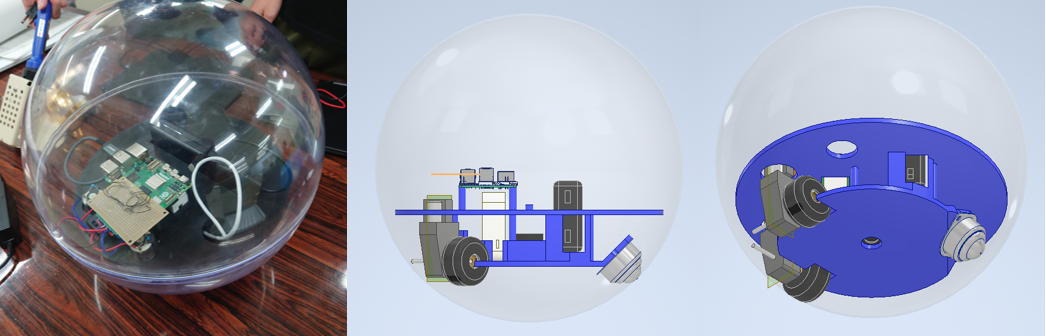
\includegraphics[width=1\hsize]{line-tracer/fig/image1.png}
  \caption{ライントレーサの外観}
  \label{fig:image1}
\end{figure}

\begin{figure}[h]
  \centering
  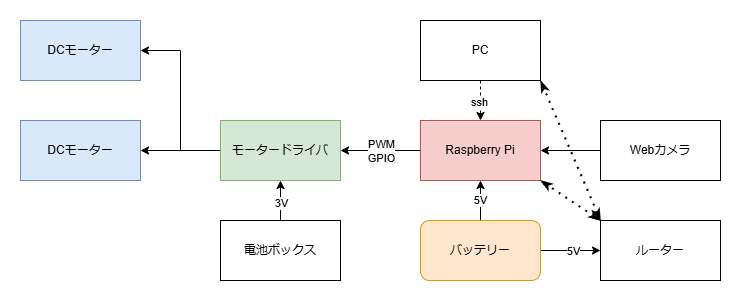
\includegraphics[width=1\hsize]{line-tracer/fig/image2.png}
  \caption{回路系システム}
  \label{fig:image2}
\end{figure}

\section{シミュレーション環境の作成}

\subsection{ランダムコース生成}
ライントレース用のランダムなコース生成は,エージェントの汎化性能を高めるために重要です。単一のコースで学習を行うとエージェントはそのコースに特化してしまい,たとえ同じコースだとしても実世界とシミュレーションのギャップに耐えられなくなってしまいます。そこで,事前に複数のランダムなコースで学習することで,様々な状況に対応できるエージェントを育成します。

コースの生成手順としては,まず領域を4×4のグリッドに分割し,幅優先探索アルゴリズムでスタート地点からゴール地点までの経路を生成します。その後,マスの境界のランダムな位置に線を通すポイントを定め,OpenCVの関数を用いて黒線を描画することでコースを完成させます。その様子を図\ref{fig:image3}に示しています。

\begin{figure}[h]
  \centering
  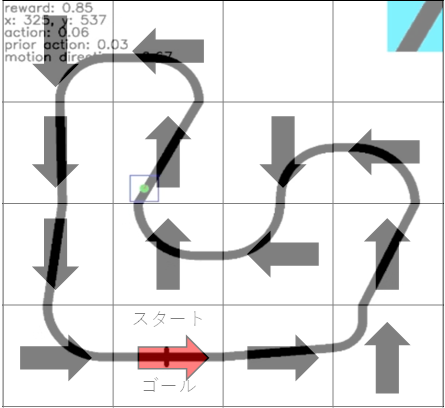
\includegraphics[width=0.7\hsize]{line-tracer/fig/image3.png}
  \caption{コース生成のイメージ}
  \label{fig:image3}
\end{figure}

\subsection{アクションの適用}
エージェントから出力されたアクションは,仮想的なライントレーサの移動方向に変換されます。初期モデルでは,アクションを2次元ベクトルで表現していましたが,コースの途中で停止したり,逆走する等の問題があり,最終的には速度を固定し自由度を削減することで,1次元のスカラーで移動方向を表現する方法を採用しました。

具体的には,図\ref{fig:image4}のように,アクション\textit{action}と概念的な進行方向\textit{action\_average}を用いて,移動方向$\theta$を計算します。なお,\textit{action\_limit}は進行方向に対して,移動方向がどれだけ逸脱できるかを制御するパラメータです。
\[
\theta = (\text{action\_average} + \text{action} \times \text{action\_limit}) \times \pi
\]
これにより,基準方向と移動方向が分離され,エージェントの学習効率が向上するとともに,前述の問題を解決することができました。
\begin{figure}[h]
  \centering
  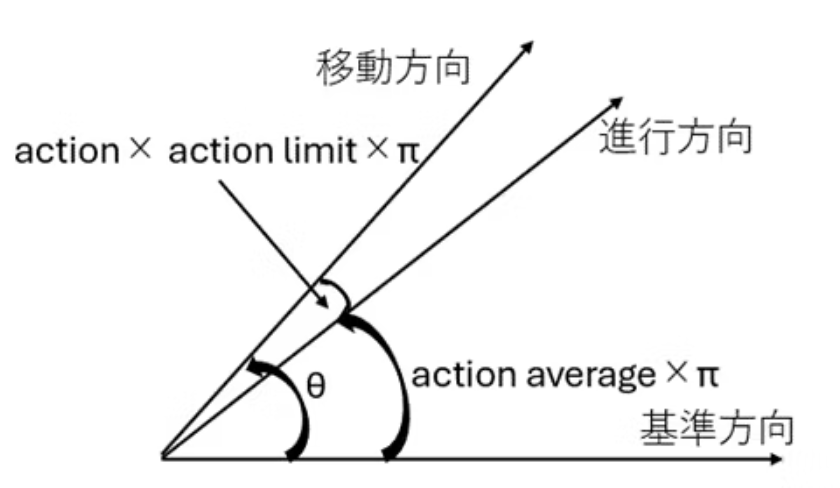
\includegraphics[width=0.7\hsize]{line-tracer/fig/image4.png}
  \caption{移動方向の計算}
  \label{fig:image4}
\end{figure}

\subsection{観測の作成}
本シミュレータでは,エージェントが観測する情報として,ライントレーサ周辺のコースを切り取った64×64のグレースケール画像,進行方向を示すスカラー値,前回のアクションを示すスカラー値の3種類を使用しています。

ただし,Gymの仕様上スカラー値も一度画像に変換し3チャンネルの画像としたうえで,エージェント側に渡しています。

\subsection{報酬関数}
報酬関数は,エージェントの行動を適切に誘導するために設計されます。今回の報酬は2つの要素から構成されています。1つ目は,前回のアクション\textit{previous\_action}とのL1誤差に基づく報酬で,アクションの振動を抑制するために設けられています。2つ目は,観測画像の中心\textit{image\_center}と,黒ピクセル(ライン)の平均座標\textit{black\_center}との距離に基づく報酬で,ロボットをライン上に維持することを目的としています。

\[
\text{reward} = 1 - \frac{| \text{previous\_action} - \text{action} |}{2} - \frac{\| \text{black\_center} - \text{image\_center} \|}{\| \text{image\_center} \|}
\]
これにより,エージェントはライン上をスムーズに移動し続けるように学習します。

\section{エージェントについて}

\subsection{活性化関数と最適化手法の変更}
今回エージェントとして採用したDrQ-v2\cite{yarats2021masteringvisualcontinuouscontrol}は,Metaが開発したQ学習ベースの強化学習アルゴリズムであり,画像を観測として連続値制御が可能な点や処理が軽量である点が特徴です。しかし,2021年の発表以降の技術進歩を踏まえ,今回の実装では活性化関数と最適化手法を変更しました。

まず,DrQ-v2では全ての活性化関数がReLUでしたが,現在はGELUやSiLUが主流です。そこで,画像処理に関わるエンコーダ部分の活性化関数をSiLUに,その他の部分はGELUに変更しました。また,最適化手法もAdamからWeight Decayを導入したAdamWに変更し,パフォーマンスと安定性の向上を図りました。

\subsection{画像とスカラーの同時入力への対応}
DrQ-v2は画像入力を前提としていますが,今回のタスクでは環境から取得した3チャンネルの画像のうち2チャンネルはスカラー情報に過ぎません。これをそのまま画像として処理するのは非効率であるため,エンコーダ部分を改良し,スカラー情報を適切に処理できるようにしました。

具体的には,画像データの内スカラーの情報しか持たない2チャンネルはスカラー値として,CNNには通さずそのまま画像の潜在表現に結合しました。この変更によって,より効率的な学習が可能となりました。

\subsection{パラメータ数の削減}
DrQ-v2の元々のパラメータ設定は複雑なタスクを想定していたため,今回のライントレースタスクに対しては過剰でした。そのため,エンコーダやアクタークリティックのパラメータを削減し,重みのファイルサイズを75158kBから3278kBへと削減しました。

結果として,図\ref{fig:image5}に示すように,若干の劣化が見られるもののモデルは十分な性能を維持しており,Raspberry Pi 5上での制御周期を1Hzから3Hzまで向上させることができました。
\begin{figure}[h]
  \centering
  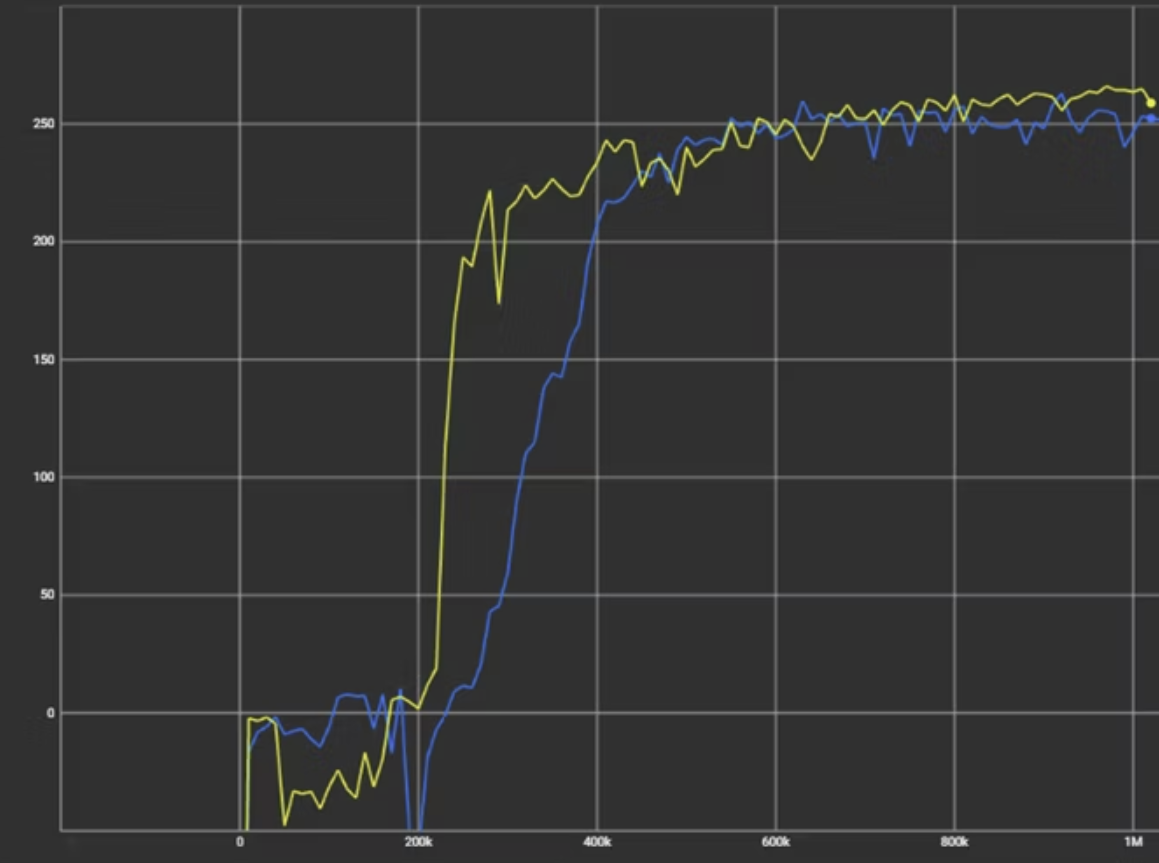
\includegraphics[width=0.7\hsize]{line-tracer/fig/image5.png}
  \caption{報酬の推移(黄色: 変更前のモデル, 青: 変更後のモデル)}
  \label{fig:image5}
\end{figure}

\section{Sim2Real}

\subsection{モータの制御}
シミュレータ上でトレーニングしたモデルを現実世界に持ってくるにあたっては,その差異をどのように減らすのかであったり,埋め合わせるのかということが重要になります。そのため今回のライントレーサは,できるだけシミュレータ上でエージェントの汎化性能を高めたうえで,現実世界の観測をシミュレータの観測に近づけるという方針で実装しました。

強化学習モデルから出力されたアクションは,前述の方法で移動方向$\theta$に変換されます。この移動方向を基に,2つのモータの回転方向とduty(出力比率)を計算し,モータードライバの制御テーブルに従ってGPIOを制御します。GPIOの制御にはRaspberry Pi用のライブラリである\texttt{gpiozero}を使用しています。

\subsection{観測の作成}
次に観測データの作成について述べます。処理の流れとしては,まずWebカメラから取得した1920×1080×3のRGB画像を正方形にトリミングして1080×1080×3にした後,64×64×3に圧縮しています。

次に,圧縮したRGB画像を64×64×1のグレースケール画像に変換し,その画像のピクセルの値の平均$\mu$を求めています。その後,求めた平均値から動的に閾値を計算して,グレースケール画像を二値化し観測としています。
\[
\text{threshold} = \mu \times \text{thresh}
\]
\[
I_{\text{binary}}(x, y) =
\begin{cases}
255 & \text{if } I(x, y) \geq \text{threshold} \\
0 & \text{if } I(x, y) < \text{threshold}
\end{cases}
\]
こうすることで,周辺環境が多少変化したとしても自動的に閾値を調整して,安定的にラインを検出できるようになります。

\section{まとめ}
以下のURLから実機を動作させた時の映像を見る事ができます。

\url{https://youtu.be/tTh6BYUjfMs?si=XSdIw1bt-LwlgnkB}
\begin{figure}[h]
  
\includegraphics[width=0.4\hsize]{line-tracer/fig/QR.png}
\end{figure}

この章では強化学習によって動作するライントレーサについて,全体的なシステム構成や実装方法を説明してきました。

今回,私がライントレーサを製作した目的の一つは,強化学習を実世界のロボットに応用することは可能なのか,また,その過程でどのような困難があるのかを検証するためでした。その結果,シミュレーションと現実のギャップや,処理速度の問題など,普段は意識しないような難しい課題が存在することが分かりました。一方で,それらの課題を解決することができれば,現実世界でも強化学習エージェントを動作させることができました。

現在,ロボティクス領域において,今回紹介した強化学習をはじめとして様々な機械学習技術の応用が行われています。今後も,機械学習とロボティクスという二つの分野が相互に影響を及ぼし,発展していく事を願っています。

ソースコードは\url{https://github.com/Azuma413/rl_linetrace}にて公開しています。
